\documentclass[12pt, a4paper]{article}
\usepackage{caption}
\usepackage{graphicx}
\usepackage{hyperref}
\hypersetup{
    colorlinks,
    citecolor=black,
    filecolor=black,
    linkcolor=black,
    urlcolor=black
}
\usepackage{listings}
\usepackage{tikz-network}
\usepackage{amsmath, amsfonts, amssymb, amsthm}
\title{Datalogi intro}
\date{2021}
\author{Kristoffer Klokker}
\begin{document}
	\maketitle
	\clearpage
	\tableofcontents
	\clearpage
		\section{Repræsentation af tal}
			Bit - 0 / 1\\
			Byte = 8 bits - 0 - 255\\
			\subsection{Konvetering fra 2 tals system til 10 tals system}
				$1011_2\rightarrow 11_{10}$\\
				\begin{align*}
					&1&&0&&&1&&&&1\\
					&1\cdot2^3&&0\cdot 2^2&&&1\cdot 2^1&&&&1\cdot 2^0\\
					&8&&0&&&2&&&&1\\
					&=11
				\end{align*}
			\subsection{Konvetering fra 3 tals system til 10 tals system}
				$1202_3\rightarrow 47_{10}$\\
				\begin{align*}
					&1&&2&&&0&&&&2\\
					&1\cdot3^3&&2\cdot 3^2&&&0\cdot 3^1&&&&2\cdot 3^0\\
					&27&&18&&&0&&&&2\\
					&=47
				\end{align*}
			\subsection{Konvetering fra hex tals system til 10 tals system}
				Grund tal for hex:\\
					$0 1 2 3 4 5 6 7 8 9 A B C D E F$\\
				$A32B_3\rightarrow 47_{10}$\\
				\begin{align*}
					&A&&3&&&2&&&&B\\
					&10\cdot16^3&&3\cdot 16^2&&&2\cdot 16^1&&&&11\cdot 16^0\\
					&40960&&768&&&32&&&&11\\
					&=41771
				\end{align*}
			\subsection{Konvetering fra hex tals system til 2 tals system}
				Da hex = 4 bits kan hver samling af 4 bits direkte oversættes til hex
				$2F7E_3\rightarrow 0010111101111110_{2}$\\
				\begin{align*}
					&2&&F&&&7&&&&E\\
					&2&&15&&&7&&&&14\\
					&0010&&1111&&&0111&&&&1110\\
					&=0010111101111110
				\end{align*}
			\subsection{Konvetering fra 10 tals system till 2 tals system via algoritme}
				Følgende algoritme finder cifrene fra højre til venstre i den binære representation af et positivt heltal $N$\\
				\begin{lstlisting}
X=N
While X > 0
	Next digit = rest ved heltalsdicistion X:2
	X = kvotient ved heltalsdivision X:2
				\end{lstlisting}
				Eksempel:\\
				\includegraphics[width=\linewidth]{assets/binAlgoritme.png}
				\textbf{Hvis man rammer 0 skal der tilføjes 1 og husk at vende den rigitge retning!}
			\subsection{Two's complement}
				Bruges til at beskrive positive og negative tal.\\
				Det første bit vil negativ og dermed hvis et binært tal starter med 1 vil det være negativt i denne repræsentationsform.\\
				For at skifte fortegn kan alle bits flippes og 1 adderes. Eks. \\
				$0110_2 \rightarrow 6_{10}$\\
				$1001_2+1=1010 \rightarrow -6_{10}$
			\subsection{Kommatal i binær}
				\subsubsection{Fast decimalpunkt}
					Den binær eksponent vil blive negativ efter komma med ens regne metode som normalt.\\
					Eks. $ 1.101_2 \rightarrow 1.875_{10}$ \\
					\begin{align*}
						&1.&&1&&&0&&&&1\\
						&1\cdot2^0&&1\cdot 2^{-1}&&&0\cdot 2^{-2}&&&&1\cdot 2^{-3}\\
						&1&&\frac{1}{2}&&&0&&&&\frac{1}{8}\\
						&=1\frac{5}{8}=1.625
					\end{align*}
				\subsubsection{Flydende decimalpunkt}
					For det flydende decimalpunkt $-9.87\cdot10^{-2}$\\
					Er eksponenten -2 og mantissen er 9.87 og den har et negativ fortegn.\\
					For 8 bits er der afsat følgende bits til at beskrive et flydende decima ud fra pensum: 1, 3 og 4\\
					Første bit er til fortegnet hvor 1 er negativt og 0 er positivt.\\
					De næste 3 er eksponent i binært\\
					De sidste 4 er til mantissen, hvor den fyldes op med 0, hvis mantissen ikke udfylder alle 4. Her vil det sidste bit i tallet også undlades da det ikke er nødvendigt og da det altid vil starte med 1.\\
					Da i det givende eksempel mantissen er for stor til 4 bits kan half-precision bruges som tager udgangspunkt i 16 bit med fordellingen: 1,5 og 10.\\
					Dermed bliver $-9.87\cdot 10^{-2}$ til $1|10010|1110110110$\\
					I tilfælde hvor mantissen ikke fyldte alle bits ville der bare fyldes 0 på i slutningen, da det blot giver en større præcision og ikke påvirker tallet.\\[8mm]
					Dette kan også bruges fra fast decimal i binært til flydende decimal, eksempelvis $-0.01101_2$\\
					Her er fortegnet negativt og dermed 1\\
					Eksponenten vil laves til -2 dermed 110 i two's complement for at det bliver negativt\\
					Mantissen er 1101, men da det første cifre altid vil være 1 undlades den\\
					Dermed bliver det $1|110|1010$
		\section{Gates og memory}
			\subsection{Gates}
				\includegraphics[width=\linewidth]{assets/gates.jpg}
			\subsection{Memory}
				A memory can be made with gates, called flip-flop\\
				\includegraphics[width=\linewidth]{assets/memory.png}
		\section{CPU}
			\subsection{Opbygning}
				ordlængde + antal bits pr manipulation typisk 32 elelr 64.\\
				\includegraphics[width=\linewidth]{assets/cpu.png}\\
				Kommando typer - flytning og manipulation af memory og ændring af program flow\\ 
				CPU cycle - Fetch (get command), decode (interpretate command), execute\\
				Program flow - styret af counter (nuværende command) og instruction pointer (næste command) som er en register\\
				En commands opbygning er først en opcode, som er et antal bits som repræsentere en command, herefter er de resterende bits argumenter.
		\section{Algoritmer}
				An algorthm is an ordered set of unambiguas executable steps that define a terminatiry process.\\
				Ofte beskrevet med pseudokode\\
				\subsection{Binary search}
					An algorythm which search thorugh an array.\\
					\begin{lstlisting}
BinarySearch(L,x)
l:=1, r:=L.lenght, m:=(l+r)/2
while l <= r and L[m]!=x
	if x < L[m]
		r:= m-1
	else
		l:=m+1
	m:=(l+r)/2
	if l <= r
		Return m
	else
		Return "Not found"
					\end{lstlisting}
					Efter 1 check vil der være $\leq \frac{n}{2^i}$ elementer tilbage. Værste tilfældet vil der være 1 tilbage i listen.\\
					$\frac{n}{2^i}<i\iff n<2^i\iff \log_2(n)<i$\\
					Dermed er køretiden O(log n)
				\subsection{Køretid}
					Køretid findes ud fra den karakteristerende operation som er propationel med køretiden.\\
					Til at beskrive køretid bruges $O(n), O(n^2)$ og lign. hvor at den enkelte algoritmes køretid vil beksrives som $T(n),T(n^2)$\\
					Her bruges $T$, da den er defineret som den tilsvarende $O$ multipliceret med en konstant.\\	
					$T(n)\in O(f(n)) \iff \exists k,m \in \mathbb{Z}:\forall n \in \mathbb{Z}, n\geq m : T(n)\leq k\cdot f(n)$
				\subsection{Invariant}
					Invariant er en måde hvorpå man kan skabe et logisk overblik over en algoritme ved brug af matematiske udtryk.\\
					Eksempelvis ved en binary search vil, invarianten være "Hvis $x$ findes i $L$, findes den i $L[l..r]$"
		\section{Merging and hashing}
			\subsection{Datastrukture}
				Datastruktur er metoder til at hente og gemme data.\\
				Interface er en række af metoder til at håndtere dataen\\
				Der er to grundtyper af interfaces Sekventiel og random access.
				\subsubsection{Sekventiel tilgang}
					Sekventiel interface håndtere data i en lang stream som et dokument.\\
					Her er metoder som, writeNext(), open(), close(), endOfFile(), readNext(), osv.\\
				\subsubsection{Random access}
					Data er gemt i et område, med en tilhørende ID.\\
					Metoder: findElm(ID), sertELM(id, data), deleteELM(ID), open(), close(), osv.
				\subsubsection{Merging}
					Merging er en teknik, hvor to sorteret lister bliver merged. Her bliver det første element fra begge altid sammenlignet og det mindste blvier taget ud og sat i den nye sorteret list.\\
					Køretiden er her $O(\log(n)n)$ grundet hvor n er størrelsen på samtlige elementer og da der bliver færre pr. itteration vil den ikke køre $O(n^2)$ men $O(\log(n)n$.\\
					Ved ikke allerede sorteret lister, vil alle elementer blive skilt ad, til lister med 1 element, hvorefter de blvier parret op.
				\subsection{Hashing}
					Hashing er en metode brugt til at vaildere filer og lign. Her kan et hashing metode bruges, hvor dataen bliver komprimeret ned, til en mindre mængde af data, hvor den kan bruges som valdiering til nye filer der blvier komprimeret ned.\\
					Den mest simple hashing metode er, at tage en array med en given st'rrelse, og på alle keys i den nye data, vil de blive udregnet $\text{key}\%\text{hast size}$. Her vil hvert element så blive indsat på den nye plads. Dette vil dog resultere i overlap, som kan ordnet på forskellige måder med den mest simple chaining som er at lave en array med element værdi og addresse til en ny array med element og addresse til den næste osv.
					En hashing metode vil ikke kunne regnes tilbage og kan derfor kun bruges til validering og ikke komprimering alene.
					\subsubsection{Sandsynlighed for overlap}
						$S_n=s_{n-1}\cdot \frac{L-(n-1)}{L}$
						Hvor L er hash længden.
		\section{Machine Learning}
			Agent a software.\\
			An agent is learning if it improves its performance by observation.\\
			Machine learning is usefull for
			\begin{itemize}
				\item Non anticipated possible solutions
				\item Non anticipated solution over time
				\item No programmable solution
			\end{itemize}
			\subsection{Forms of machine learning}
				Supervised learning - Learns from problems with solutions and apply them to future problems. Ex. housing pricing.\\
				Unsupervised learning - Problems have no real solution but rather categorize data. Ex. Categorizing Amazon users in buying habits.\\
				Reinforcement learning - Rule judges if agent is right or wrong from which it learns. Ex. AI learns games
			\subsection{Supervised Learning}
				Input = features\\
				Output = responses\\
				Learning is based on $m$ input vector with all features where it is a set with $\{(\vec{x_1},y_1),(\vec{x_2},y_2),...,(\vec{x_m},y_m)\}$\\
				From learning it will generate a function $g(\vec{x})$ from which $g(\vec{x_m})\approx y_m$\\
				$\hat{y}=g(\vec{x})$
				\subsubsection{Regression problem}
					Used to predict a quantitative solution\\
					Nearest neightbor - Takes the nearest points to the given $x$ values and returns the average $\hat{y}=\frac{1}{k}\sum\limits_{\vec{x_i}\in N_k(\vec{x})}y_i=g(\vec{x})$\\[5mm]
					To find the best function in a 2 dimensional regression a loss/error function can be defined as $\hat{L}(a,b)=\sum\limits_{i=1}^m(y_i-ax_i-b)^2$\\
					The more general loss for the poly function is $$\hat{L}(\vec{\theta})=\sum\limits_{i=1}^m(y_i-h(\vec{\theta},\vec{x_i}))^2=\sum\limits_{i=1}^m(y_i-\sum\limits_{j=0}^p\theta_jx_{ij})^2$$
					Where $h(x)=poly(\vec{\theta},x)=\theta_0+\theta_1x+...+\theta_kx^k$\\
					The functions distance can be squared or absolute to counter negative variation and squared to make higher values more important.\\
					From this partial differential can be used where one value is constant and the differentiation is found and set equal to zero to find one constant.\\
					From this the other constant can be found through differentiation and finding it when equal zero. This is done until all variables are found.\\
					With this technique a local optimum for the lowest error.
				\subsubsection{Classification problem}
					used to predict qualitive (binary) solution
					Nearest Neightbor - Just like regression but instead of average, it takes the majority
			\subsection{General framework}
				Learning = Representation + Evalutation + Optimization\\
				Representation: How input is represented. Ex. the hypothesis set for regression problems\\
				Evaluation: Defining the loss function\\
				Optimization: Finding the best learner in the language for minimizing the loss
			\subsection{Overfitting}
				Overfitting is the act of using a too high $k$ value in the poly regression. Here a too high value will end up hitting all data, but as a result most likely not represent the actual underlying function.
			\subsection{Training and Assessment}
				To ensure not overfitting the training methods can me used. Here there are two techniques.\\
				\begin{itemize}
					\item Holdout method - Using only 75\% ish for training and 25\% for testing
					\item K-fold cross validation - Used in small data, where samples of the training data is used for testing
				\end{itemize}
			\subsection{McCulloch-pitts "units"}
				\begin{center}
					\includegraphics[width=300px]{assets/neuron.png}
				\end{center}
				$a$ is input\\
				$w$ is weights\\
				The comparing can also be made an input is $a_0$ and instead it compares to 0.\\
				Instead of comparing to 0 an activation function can be used. This will make it derivable to find the minimum.\\
				The most comman is the sigmoid function $\frac{1}{1+e^{-x_i}}$\\
				Neurons are able to replicate boolean functions and therefore opens neurons possibilities a lot.\\
				Though the XOR is not directly possible due to it not being possible to create a activation function which includes (0,1) and (1,0) but not (0,0) and not (1,1).
			\subsection{Network structures}
				Structure(/Architecture): defnition of number of nodes, interconnections and activation functions $g$ (but not weights).
				Two types of structures Feed forward netorks and Recurrent networks\\
				Feed-forword netowrk has no cycles and can be single-layer (no hidden layer) or multi-layer perceptrons (hidden layers). Used in classification and regression.\\
				Recurrent networks has cycles between nodes which result in possible memory in the network\\
				Multiplayered perceptrons have hidden units typically choosen by hand\\
				With more layers the threshold function will combine meaning a more precise threshold
		\section{Reature spaces for repesentation of images}
			Features are ways to describe an image such as color distribution, shapes and so on.
			\subsection{Color histogram}
				Color histograms are used to represent the distrubution of colors.\\
				here each color is distributed into intensity and then normalised with the total pixels used.\\
				Here the amount of distribution determine the amount of compression.\\
			\subsection{Distance of color histograms}
				Euclidean distance - representring the histogram as a vector and using calculating the distance by subtracting every points and multiplying them together and taking square root. Ex $$\text{dist}(P,Q)=\sqrt{(h_P-h_Q)\cdot (h_P-h_Q)}$$
				Psychologic distance - takes in measures such as pink and cyan being close together as colors and weights that higher.\\
				Distance can also be measured in different ways, for example let it be a classification problem the distance can be  $$\text{dist}_P(p,q)=w_1(|p_1-q_1|^P\cdot w_2|p_2-q_2|)^{\frac{1}{P}}$$ Where $w$ is the different weights.\\
				Here if $P=2$ we get the distance formula from before. Different $P$ values will here create different shapes of classification. The different shapes can be seen on the picture with 1 distance unit between the two black lines.\\
				\begin{center}
					\includegraphics[width=\textwidth]{assets/distanceFormula.png}\\
					Left - $L_2$ \\
					Middle - $L_1$\\
					Right - $L_{\infty}$\\
					As seen the higher $P$ values results in the corners being included.
				\end{center}
				
		\section{Clustering}
			Clustering is used to categorize data.\\
			Good clustering will have an amount of clusters which will result in furthest distance between clusters and shortest distance between point and clusters.\\
			There are algorithms which will help clustering data points.\\
			\subsection{Lloyd/forgy}
				Assign all points random clusters.\\
				Calculate the mean point of all clusters.\\
				Assign each point to closest cluster.\\
				Recalcluate mean cluster points.\\
				Repeat until no change.\\
			\subsection{MacQueen/$k$-means}
				Assign all points random clusters\\
				Calculate mean cluster points\\
				In a given order assign an element to closest cluster point and recalculate cluster mean points.\\
				Repaeat last step until no change.
		\section{Models of Computation, languages and Recursion}
			\subsection{Models of Computation}
				Models of computation are ways of working with problems the most effective way\\
				The models focus on important parts of problems and sort out unimportant parts\\
				Example compilers how the first took centuries to develop and today is a simple project.
			\subsection{Deterministic Finite Automaton (DFA)}
				DFA is a way of illustrating regular expressions via graphs.\\
				Forexample $[He+y]$ will be:\\
				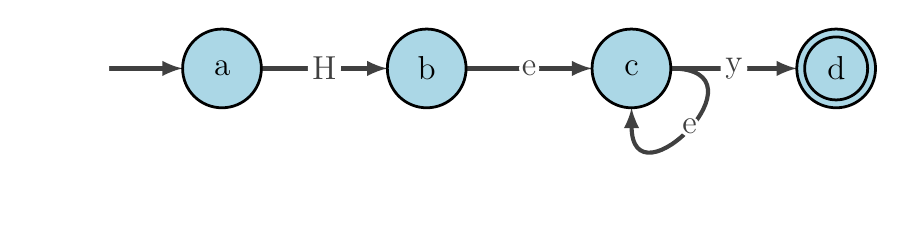
\begin{tikzpicture}[scale=1.3]
					\SetVertexStyle[MinSize=1\DefaultUnit,TextFont=\large]
					\SetEdgeStyle[TextFont=\large]
					\Vertex[x=0,style={color=white}]{Z}
					\Vertex[label=a,x=1.5]{A}
					\Vertex[label=b,x=3.5]{B}
					\Vertex[label=c,x=5.5]{C}
					\Vertex[x=7.5]{D}
					\Vertex[label=d,x=7.5, size=0.8]{O}
					\Edge[Direct](Z)(A)
					\Edge[Direct,label=H](A)(B)
					\Edge[Direct,label=e](B)(C)
					\Edge[Direct,label=y](C)(D)
					\Edge[Direct,label=e,loopposition=-45](C)(C)
				\end{tikzpicture}\\
				The double ring at d illustrates a acceptence state, inwhich a DFA ends.\\
				An edge can have multiple poosibilites but not the same.\\
				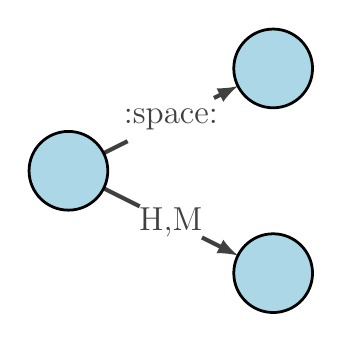
\begin{tikzpicture}[scale=1.3]
					\SetVertexStyle[MinSize=1\DefaultUnit,TextFont=\large]
					\SetEdgeStyle[TextFont=\large]
					\Vertex[x=0,y=1]{A}
					\Vertex[x=2]{B}
					\Vertex[x=2,y=2]{C}
					\Edge[Direct,label={H,M}](A)(B)
					\Edge[Direct,label=:space:](A)(C)
				\end{tikzpicture}\\
				The : notation is used to describe groups of characters or not visible.\\
				Concatenation is combining multiple DFAs\\
				DFAs are limited, one example is the langauge made of $($ and $)$ which always has to matched.\\
				Here the DFA has to be endless, to compensate for an endless string of $($ and $)$.
			\subsection{Conttext-Free Grammar}
				CFG is a rule based regex. Here characters is terminals and regex applications (possibilites) are called deriviations\\
				Example:\\
				S $\rightarrow$ Hello T\\
				S $\rightarrow$ Hey T\\
				T $\rightarrow$ there\\
				It will here insert rules if given in the string of a rule.\\
				The deriviations are: Hey there og Hello there\\[4mm]
				CFG is able to store memory using recursion. To describe the language of matched parenthesis like the DFA not could it would be.\\
				S $\rightarrow$ (S)\\
				S $\rightarrow$ SS\\
				S $\rightarrow$ ()\\
				By recursionit will be able to go to the closing parenthesis after an opening.
		
		\section{Online aglrithmes}
			Algorithms based on unexpected data. Unlike offline data where data is known and the algorithm can be optimized based on data online algorithms has to oprimize for the unknown.\\
			An algorithms competitive is the ratio between offline and online performance. From which the c-compeittive ratio is $\forall I: \frac{ALG(I)}{OPT(I)}\leq C$.\\
			Therefore an algorithms ratio is the ratio between the online and offline guarantee worst case for an algorithm.\\
			An example is computation qeue algorithms which gives computations to $m$ computers. \\
			The offline version can see all the data and optimize for all the data, and the online version will only see the next data.\\
			The online algorithm can here be given the computer with the least amount of work the next computation.\\
			The ratio can here be proofed by the following:\\
			\begin{center}
				\includegraphics[width=300px]{assets/onlineAlg.png}
			\end{center}
			$t$ is the last job\\
			$l$ is the length of the lowest job before $t$\\
			$T$ is the total length of all job\\
			$V=l\cdot m$\\
			OPT$\geq T/m$ and OPT$\geq t$\\
			$T\geq v+t$\\
			\begin{align*}
				\text{L}_S=&l+t\\
						&\geq \frac{T-t}{m}+t&&\text{since}\; l=\frac{V}{m} \;\text{and}\; V\geq T-t\\
						&=\frac{T}{m}+(1-\frac{1}{m})t\\
						&\geq \text{OPT}+(1-\frac{1}{m})\text{opt}&&\text{since OPT$\geq T/m$ and OPT$\geq t$}\\
						&=(2-\frac{1}{m})\text{OPT}
			\end{align*}
			
		\section{Satisfiability}
			A propositional formula is satisfiable if variables can be assigned such it returns true.\\
			By describing problems via propositional formulas, it can be solved by SATs.\\
			A SAT is a program which can find solutions for propositional formulas.\\
			To use a SAT the formula has to be CNF by:\\
			\begin{itemize}
				\item $F\rightarrow G = -F\lor G$
				\item $-(F\land G) = -F\lor -G$
				\item $-(F\lor G) = -F \land -G$
				\item $-(-F)=F$
				\item $F\lor (G\land H) = F\lor G)\land (F\lor H)$
			\end{itemize}
			For a SAT input lines beginnings are compiled as:
			\begin{itemize}
				\item p - Problem formatted as $p\; cnd\; \#variable\; \#cause$
				\item c - comment
				\item s - output for solutuion
				\item v - variable assignment from output
			\end{itemize}
			Lines are OR'ed and rows are AND'ed.\\
			SAT solving is based on trying every possible solution\\
			This is optimized by:
			\begin{itemize}
				\item Incremental assignments
				\item Backtracking solver
				\item Pruning the search
				\item Backjumping
				\item Conflict-driven learning
				\item Restarts
				\item Forgetting
			\end{itemize}
		\section{Databaser}
			Databases are a software tool to store and organize large amount of data.\\
			Data can be accessed by multiple users and data are enforced by constraints.
			DBMS - database management systemt\\
			Modern DBMS - helps with backup, permission, consistency, searching sorting filtering, multi-users\\
			There are to types of DBMS\\
			Data entries are called tuple
			\begin{itemize}
				\item Relational DBMS - Table system with data
				\item Graph DBMS - Directional graph good to see patterns
			\end{itemize}
			A database is structured as:
			\begin{itemize}
				\item Conceptual - ER diagram
				\item Logical - Relation diagram
				\item Physical - SQL language
			\end{itemize}
			\subsection{Conceptual}
				Entity-relationship (ER) diagrams\\
				$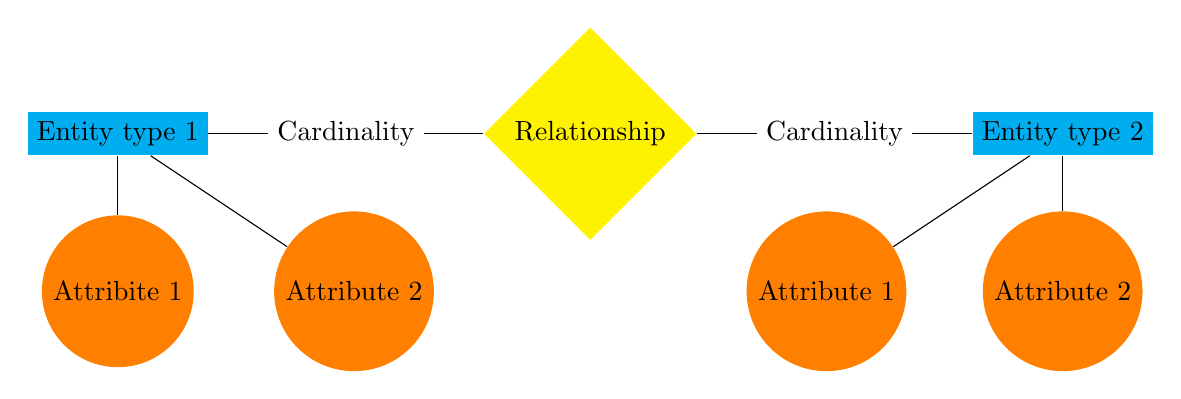
\begin{tikzpicture}[scale=2]
					\node[fill=cyan](v1) at (0,1){Entity type 1};
					\node[fill=yellow,diamond](v2) at (3,1){Relationship};
					\node[fill=cyan](v3) at (6,1){Entity type 2};
					\node[fill=orange,circle](v4) at (0,0){Attribite 1};
					\node[fill=orange,circle](v5) at (1.5,0){Attribute 2};
					\node[fill=orange,circle](v6) at (4.5,0){Attribute 1};
					\node[fill=orange,circle](v7) at (6,0){Attribute 2};
					\path[-]
						(v1) edge node {}(v4)
						(v1) edge node {}(v5)
						(v3) edge node {}(v6)
						(v3) edge node {}(v7)
						(v1) edge node[fill=white] {Cardinality}(v2)
						(v2) edge node[fill=white] {Cardinality}(v3);
				\end{tikzpicture}$\\
				Cardinality describes the amount of relation. Ex. 1..n mean there must be at least 1 to n amount in the given relation.\\
				Relation - describes the relation between two entities: Ex. owns\\
				Relation can also have attributes such as date of ownership.\\
			\subsection{Logical}
				Here the tables are somewhat esatablished\\
				This is through:\\
				$relation_{name}(attribute1,attribute2,...)$ or\\
				$relation_{name}(attribute1: type1,...)$\\
			\subsection{Physical}
				The SQL command level\\\
				Remember string must be with ' and not "\\
				The usal commans $CREATE$, $INSERT$, $DELETE$, $SELECT, FROM, WHER$
				\subsubsection{Relatio Algebra}
					$\sigma_c(R)$ Selection - gather rows with the given $c$ condition\\
					$\pi_{A_1,..A_k}$ projection - gather columns $A_1,..A_k$
					All of the usual set operators $\cup,\cap,\times ...$
			\subsection{Integrity Constraints}
				Constraints is in form of data types and size limit\\
				This is things such as name begin $CHAR(20)$\\
				The ensure data integridy
			\subsection{Primary key}
				Column with data which is uniqe data.\\
				Can not have duplicate to ensure data integridy
		\section{Cryptology}
			The science of cryptologi is in two genres:\\
			Cryptography is written something hidden\\
			Crypanalysis is braking cryptography\\
			The goal of cryptography is securing 
			\begin{itemize}
				\item confidentilly to secure encryption
				\item Integrity is often done thorugh hash keys which verify the message
				\item Authenitcy is also a part of integrity
				\item Non-repudiantion is important so its validated that a message actually was sent
			\end{itemize}
			\subsection{Encryption}
				Encryptions goal is to have a key which maps the messages and is bijections so decryption is possible\\
				Message space is the readable message and cipher space is the encrypted format\\
				The most simple is ceasar sipher which mapping shift all charachters by the key number\\
				The problems is bruteforcing is pretty easy with only 29 keys.\\
				A good number is $2^{128}$ for amount of keys so its not bruteforceable\\
				Kerckhoffs's Principle - The security should rely in the key and not the system\\
				Vigenére Cipher - Ceasar cipher but with a rotating key such as $314$\\
				One-Time-Pad - using a non repeating key but an infinite long key\\
				The problem is integrity is hard to ensure no bit flip and sharing the key is hard\\
				A good way to analyse different encryption methods is images, which is easy to find patterns in.\\
			\subsection{Symmetric key systems}
				Symmetric - both sides has the same key.\\
				\begin{itemize}
					\item Caesar cipher
					\item Enigma
					\item DES - had only $2^56$
					\item Tiple DES - had $2^112$ but it was a combination of DES which resulted in flaws
					\item AES - $2^{128}$ or $2^{256}$ keys and currently not bruteforceable, worked since 2001 and standard today
				\end{itemize}
			\subsection{Assymtric keys}
				To counter the problem with two people having the same key a private key and public key is used\\
				People sending a message to a person they encrypt it with the persons public key\\
				Then it is decrypted with the private key\\
				Here the private key has to be hard to find out both from bruteforce or reverse engineering the prublic key.\\
			\subsection{RSA}
				$N_A=p_A\cdot q_A$ where the right side is primes\\
				$gcd(e_A,(p_A-1)(q_A-1))=1$\\
				$e_A\cdot d_A\equiv 1$ (mod$(p_A-1)(q_A-1))$.\\
				Public key $PK_A=(N_a,e_A)$\\
				Private key $SK_A=(N_A,d_A)$\\[4mm]
				To encrypt:\\
				$c=E(m,PK_A)=m^{e_A}$ (mod $N_A$)\\
				To Decrypt:\\
				$r=D(c,SK_A)=c^{d_A} $ (mod $N_A$).
				\subsubsection{Why it works}
					We want to proof that $r=(d(E(m,PK_A)SK_A)$\\
					We know that $e_Ad_A=1+k(p_A-1)(q_A-1)$\\
					\begin{align}
						r&\equiv(m^{e_A}\;(mod\;N_A))^{d_A}\;(mod\;N_A)\\
						 &\equiv m^{e_A^{d_A}}\;(mod\;N_A)\\
						 &\equiv m^{e_A\cdot d_A}\;(mod\;N_A)\\
						 &\equiv m^{1+k(p_A-1)(q_A-1)}\;(mod\;N_A)
					\end{align}
					1. first we insert the definition on encryption and decryption.\\
					2. This is then reduced\\
					4. Then the definiiton of $e_a\cdot d_A$ is inserted\\
					\begin{align}
						r&\equiv m^{1+k(p_A-1)(q_A-1)}\;(mod\;p_A)\\
						 &\equiv m\cdot (m^{(p_A-1)})^{k(q_A-1)}\;(mod\;p_A)\\
						 &\equiv m\cdot 1^{k(q_A-1)}\;(mod\;p_A)\\
						 &\equiv m\;(mod\;p_A)
					\end{align}
					5. We then ise $p_A$ instead of $N_A$\\
					6. We then rewrite\\
					7. By fermats little rule we we know that $m^{(p_A-1)}\;(mod\;p_A$ is equivalent to 1\\
					8. We then reduce by everything to the power of 1 is 1\\
					We see in case we use $q_A$ instead of $N_A$ like with $p_A$ it will result in the same result $r\equiv m\;(mod\;q_A)$
					We can then use chinese remainder theoroem due to $gcd(p_A,q_A)=1$\\
					\begin{align*}
						r&\equiv m\;(mod\;p)\\
						r&\equiv m\;(mod\;q)\\
						N=pq\\
						r\equiv m\equiv m\;(mod\;N)\\
						r\equiv m\;(mod\;N)
					\end{align*}
					This means $m$ can be everything due to $m$ always will be equivalence to $m$\\
					And since $r$ is equivalent to $m$ mod $p,q,N$ and $r$ and $m$ can not be larger than $N-1$ must therefore be equal $r=m$
				\subsubsection{Why RSA is secure}
					Well to decrypt a text given $c$ and $PK_A=(N_A,e_A)$, it has to find
						$$c=m^{e_A}\;(mod\;N_A)$$
					Which there is no simple algorithm to solve and bruteforce is needed.\\[4mm]
					To ensure a private key is not found the factoring of $N_A$ must be hard.
					To bruteforce $N_A$ if a single prime is known it will only take $O(\sqrt{N})$ time
					This means if $N$ is 3072 bits it will take almost forever.\\
					if the length is $n=\lceil \log_2(N+1)\rceil$ the run time will be $O(2^{n/2})$\\
					But it may not be true due to quantum computers can have more effecient algorythm\\
				\subsubsection{RSA implementation}
					To implment RSA for the encryption part the expression $a^k$ (mod n) is used.\\
					If done as said there would be $k-1$ modular multiplications, which is too many\\
					This can be optimized by a recursive function where if the power is odd its possible to minus 1 from the exponent  and multiply, and if even it can be halfed and multiplied. RSA program implements this for more detail.\\[4mm]
					To find $e_A$ and $d_A$ the following expression has to be used\\
					$$gcd(e_A,(p_A-1)(q_A-1))=1$$
					$$e_A\cdot d_A\equiv 1\;(mod\;(p_A-1)(q_A-1))$$
					This can be done with the extended Euclidean algorithm\\
					This can find $d_A$ through the gcd. The algorithm is implemented in the RSA program.\\[4mm]
					To find prime numbers there are a number of different ways\\
					\begin{itemize}
						\item Sieve of Eratosthenes - Take all numbers the first in the list is a prime and after removing it remove all multiples
						\item Bruteforce - Take all numbers from 0 to $\sqrt{n}$ and test if it divides with the prime
						\item Miller-Rabin test - Choose a random number from which it can be tested if Fermat test works
					\end{itemize}
					The most effective is the Miller-Rabin which is implemented in the RSA program.\\
					Carmicheal numbers are numbers which are hard to determine if composit, ex 561 where only 241 out of the 560 determine it as a composit.\\
				\subsection{Symmetric and public key system}
					To speed up RSA due to it slow nature, a symmetric session key is genereated from the RSA.\\
					Digital signatures is also implemted with RSA, by encrypting the fixed length:q
					signature with the private key and public keys can then validate if it can be decrypted.
			\section{Graph theory}
				Vertices points in graph\\
				Edges lines connecting vertices\\
				Degree number of edges on a vertice\\
				Categories of graphs
				\begin{itemize}
					\item labelled graph - vertices has names
					\item Directed graph - vertices has a direction
					\item Weighted graph - edges has an weight for moving past
				\end{itemize}
				Walks - a route on a graph which goes between two vertices\\
				Path - walk without any repetition on an edge\\
				Cycles - Closed walks\\
				Connectedness - If a number of graph is in more parts
				\subsection{Matrix representation}
					$$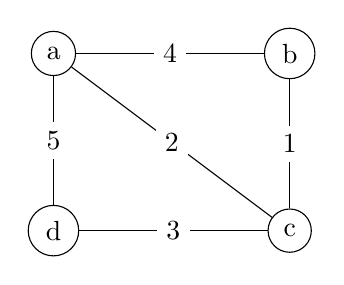
\begin{tikzpicture}[scale=3]
						\tikzstyle{vertex}=[circle,draw=black]
						\node[vertex](v1) at (0,0.75) {a};
						\node[vertex](v2) at (1,0.75) {b};
						\node[vertex](v3) at (1,0) {c};
						\node[vertex](v4) at (0,0) {d};
						\draw (v2) -- (v3) node [midway, fill=white] {$1$};
						\draw (v1) -- (v3) node [midway, fill=white] {$2$};
						\draw (v3) -- (v4) node [midway, fill=white] {$3$};
						\draw (v1) -- (v2) node [midway, fill=white] {$4$};
						\draw (v1) -- (v4) node [midway, fill=white] {$5$};
					\end{tikzpicture}$$
					\begin{minipage}{0.45\textwidth}
						Incidence Matrix\\
						Edges has labels\\
						$$\begin{bmatrix}0&0&0&0&1&1\\1&0&0&0&1&0\\1&1&1&0&0&0\\0&0&1&0&0&1\end{bmatrix}$$
					\end{minipage}
					\hfill
					\begin{minipage}{0.45\textwidth}
						Adjecency Matrix\\
						Edges has weight\\
						$$\begin{bmatrix}0&4&2&5\\4&0&1&0\\2&1&0&3\\5&0&3&0\end{bmatrix}$$\\
					\end{minipage}
						To find paths between points the adjecent matrix can be multiplied with itself $k$ ($A^k$) times where if there is a 1 there exists a path with $k$ length.\\
					For the shortest path between two points the adjecenst matrice can be multiplied but instead of multiply plus is used and instead of plus the minimum of the sums is choosen.\\
					It then has to be multiplied the amount of vertices -1.\\
					$w=\begin{bmatrix}0&4&2&5\\4&0&1&0\\2&1&0&3\\5&0&3&0\end{bmatrix}$
					$w^2=\begin{bmatrix}0&3&2&4\\3&0&1&0\\2&1&0&1\\4&0&1&0\end{bmatrix}$
					$w^3=\begin{bmatrix}0&3&2&3\\3&0&1&0\\2&1&0&1\\3&0&1&0\end{bmatrix}$\\
					To optimize the matrice can be mutliplied by itself so for a graph with 121 vertices instead of 121 computations the matrice can be $a^{2\cdot 2\cdot 2\cdot 2\cdot 2\cdot 2\cdot 2}$
					


			
			

			
				
					
\end{document}

